\section{Expérience G2} \label{expG2}
  \subsection{Objectif}
    En utilisant la seconde architecture de \cite{Cleeremans_2007}, 
    comprendre de quelles manières un réseau de neurone connexionniste peut, à partir de ses propres paris
    sur son résultat, améliorer son comportement, à partir d'un 3\up{ème} réseau.
  
  
     
  \subsection{Architecture}
    \paragraph{Description}
      Un premier réseau de perceptron multicouche apprend à discrétiser des chiffres représentés
      par 256 (16x16) neurones d'entrées. Il est composé d'une couche cachée de 100 neurones.
      
      Un second réseau de perceptron multicouche apprend à parier sur la qualité de la réponse
      du premier réseau à partir de sa couche cachée.
      
      L'apprentissage du second réseau, n'affecte pas les poids entre la couche d'entrée et la 
      couche cachée du premier réseau.
      
      Lorsque le second réseau parie haut, la réponse du premier réseau est gardée, à l'inverse,
      lorsqu'il parie bas, c'est le second neurone le plus élevé du premier réseau qui sera 
      la réponse.
      
      Un troisième réseau de perceptron apprend la solution à partir des sorties des 2 premiers 
      réseau. Son apprentissage n'affecte aucun des 2 sous réseaux.


    \paragraph{Schéma}
      \begin{center}
	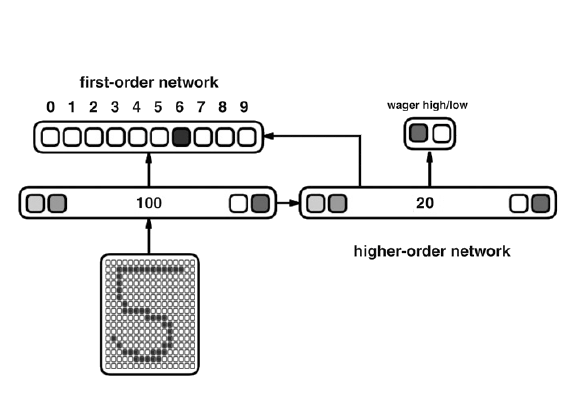
\includegraphics[width=250px]{data/expG2/schema.png}
      \end{center}
      
    \paragraph{Paramètres}
      \begin{center}
	\begin{tabular}{lr}
	  \begin{minipage}{230px}
	    \begin{itemize}
	      \item momentum : 0.5 sur le premier réseau
	      \item momentum : 0. sur le 2\up{ème} et 3\up{ème} réseau
	      \item taux d'apprentissage : 0.15 sur le premier réseau
	      \item taux d'apprentissage : 0.1 sur 2\up{ème} et \up{ème} réseau
	      \item \textbf{1600 formes} de chiffres différents présentées (shuffle) \cite{Handwritten_256}
	      
	      
	    \end{itemize}
	  \end{minipage}
	  &
	  \begin{minipage}{230px}
	    \begin{itemize}
	      \item poids initialisés sur [-1 ; 1] pour le premier réseau
	      \item poids initialisés sur [-0.25 ; 0.25] pour le 2\up{ème} et 3\up{ème} réseau
	      \item taux d'apprentissage constant
	      \item entrées valent 0 ou 1
	      \item sigmoïde à température 1
	      \item utilisation de biais
	      \item apprentissage 50 (formes) x 300 (époques)
	    \end{itemize}
	  \end{minipage}
	\end{tabular}
      \end{center}
  
  \newpage
  \subsection{Résultats}
    \paragraph{Principaux}
      Analyse des performances
      \begin{center}
	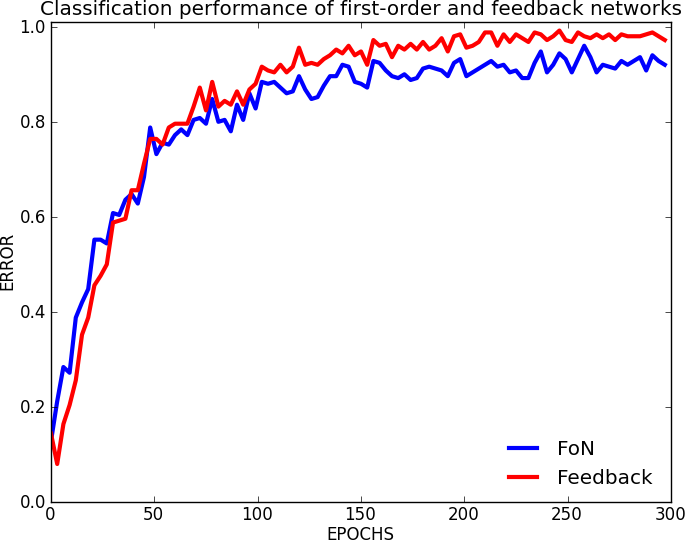
\includegraphics[width=250px]{data/expF1/perff.png}
      \end{center}
      \subparagraph{Notes}
	\begin{itemize}
	  \item La performance de classification représente le taux de bonnes réponses (winner-take-all) pour les 50 formes présentées sur une époque
	\end{itemize}
      \subparagraph{Conclusion}
	\begin{itemize}
	  \item il faut attendre les 50 premières époques pour que le 3\up{ème} réseau puisse profiter d'une hausse de performance
	\end{itemize}
    \paragraph{Secondaires}
      Analyse des performances sous-jacentes
      \begin{center}
	\begin{tabular}{lr}
	  \hspace*{-1cm}
	  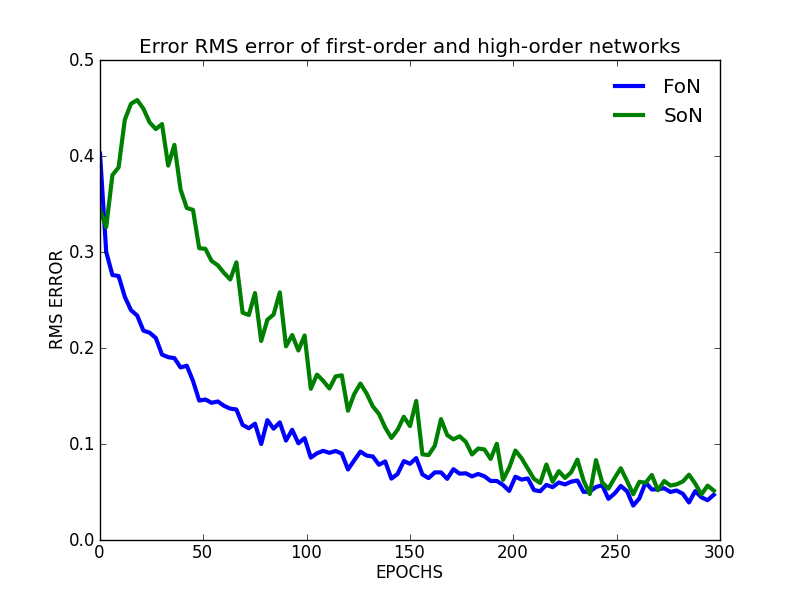
\includegraphics[width=250px]{data/expF1/rms.png}
	  &
	  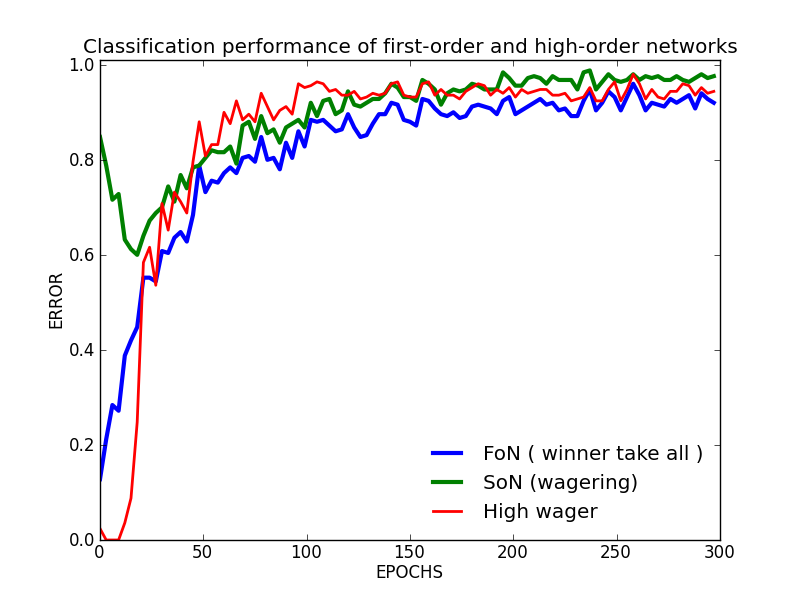
\includegraphics[width=250px]{data/expF1/perf.png}
	\end{tabular}
      \end{center} 
      \subparagraph{Notes}
	\begin{itemize}
	  \item formule utilisée pour RMS (cf. Formules~\nameref{rms})
	  \item la courbe rouge représente le taux de paris haut du second réseau
	\end{itemize}
      \subparagraph{Conclusion}
	Les bonnes performances du second réseau permettent une l'augmentation de performance du 3\up{ème} réseau.


  \subsection{Conclusion}
  La mise en place de ce 3\up{ème} réseau permet une légère hausse de performance. Il est intéressant de voir qu'uniquement
  grâce à un chiffre donné ( sortie du premier réseau ) et grâce à un paris ( sortie du 2\up{ème} réseau ), on arrive 
  quand même à avoir une hausse de performance.
  
  Pour résoudre le problème de temps d'apprentissage des 50 premières époques et du 3\up{ème} réseau supplémentaire,
  l'expérience G1.
  
  
  Évidemment, comme nous l'avons montré dans les expériences C, il faut un nombre élevé de neurone dans la couche cachée du premier réseau.
  Cette hausse de performance ne peut dépasser les performances d'un réseau optimal.
  
  

  \newpage 
  \subsection{Formules}
    \paragraph{RMS} \label{rms}
  Pour une époque $e$ :
  \begin{center}
    \begin{large}
    $ rms_{e} = \sqrt{ \frac{1}{n} \sum \limits_{i=1}^{n} 
    ( o_{i,e} - d_{i} )^2 } $
    \end{large}
  $ with \left\lbrace \begin{array}{lll} n : number\ of\ neurons\ on\ the\ output\ 
  layer\\o_{i,e} : value\ obtained\ for\ the\ i^{th}\ neuron\ at\ the\ e^{th}\ epoch\\d_{i} : 
  value\ desired \ for\ the\ i^{th}\ neuron\end{array} \right.$
  \end{center}
    
    \paragraph{Descente de gradient} \cite{Touzet_1992} \\
  Construction de l'erreur : 
    \begin{center}
      $y_{i} = f'(a_i) \times ( d_i - x_i ) \ si\ i\ neurone\ de\ sortie $ \\
      $y_{i} = f'(a_i) \times \sum \limits_{k} ( w_{ki} \times y_k )\ si\ i\ neurone\ cache $
    \end{center}
  Mise à jour des poids :
    \begin{center}
      $w_{ij}(t+1) = w_{ij}(t) + learning\_rate \times y_{i} \times x_j + momentum \times 
      (w_{ij}(t) - w_{ij}(t-1) )$
    \end{center}
  Variables : 
    \begin{center}
      $\left\lbrace \begin{array}{lll} 
	f : fonction\ sigmoide \\
	x_i : valeur\ du\ neurone\ i\\
	d_i : valeur\ desire pour\ le\ neurone\ i\\
	a_i : somme\ pondere\ des\ poids\ du\ neurone\ i
      \end{array} \right.$
    \end{center}
    
\bibliographystyle{../pre-rapport/apalike}
\bibliography{../pre-rapport/biblio}
